\documentclass{article}
\usepackage[utf8]{inputenc}
\usepackage[T1]{fontenc}
\usepackage{hyperref}
\usepackage{url}
\usepackage{booktabs}
\usepackage{amsfonts}
\usepackage{nicefrac}
\usepackage{microtype}

\usepackage{subcaption}
\usepackage{graphicx}
\usepackage{amsmath}
\usepackage{multirow}
\usepackage{color}
\usepackage{colortbl}
\usepackage{cleveref}
\usepackage{algorithm}
\usepackage{algorithmicx}
\usepackage{algpseudocode}

\DeclareMathOperator*{\argmin}{arg\,min}
\DeclareMathOperator*{\argmax}{arg\,max}

\graphicspath{{}}

\begin{filecontents}{references.bib}
@article{Cappellari2008,
  author = {Cappellari, Michele and Emsellem, Eric and Krajnovi\'{c}, Davor and others},
  title = {The SAURON project - X. The stellar mass distribution of early-type galaxies: fast rotators and slow rotators},
  journal = {Monthly Notices of the Royal Astronomical Society},
  year = {2008},
  volume = {386},
  pages = {1860-1884}
}

@article{Chabrier2003,
  author = {Chabrier, Gilles},
  title = {Galactic Stellar and Substellar Initial Mass Function},
  journal = {Publications of the Astronomical Society of the Pacific},
  year = {2003},
  volume = {115},
  pages = {763-795}
}

@article{Conroy2013,
  author = {Conroy, Charlie},
  title = {Modeling the Panchromatic Spectral Energy Distributions of Galaxies},
  journal = {Annual Review of Astronomy and Astrophysics},
  year = {2013},
  volume = {51},
  pages = {393-455}
}

@article{Suyu2006,
  author = {Suyu, Sherry H. and Marshall, Philip J. and Hobson, Michael P. and Blandford, Roger D.},
  title = {The Hubble Constant from the Gravitational Lens B1608+656: A Second Measurement},
  journal = {The Astrophysical Journal},
  year = {2006},
  volume = {644},
  pages = {330-340}
}

@article{Warren2003,
  author = {Warren, S. J. and Dye, S.},
  title = {A new method for analysing gravitational lens systems: the lens and source reconstruction algorithm},
  journal = {The Astrophysical Journal},
  year = {2003},
  volume = {590},
  pages = {673-682}
}

@article{auger2010,
  author = {Auger, M. W. and Treu, T. and Bolton, A. S. and Gavazzi, R. and Koopmans, L. V. E. and Marshall, P. J. and Moustakas, L. A. and Burles, S.},
  title = {The Sloan Lens ACS Survey. X. Stellar, Dynamical, and Total Mass Profiles of Early-Type Galaxies},
  journal = {The Astrophysical Journal},
  year = {2010},
  volume = {724},
  pages = {511-525}
}

@article{barnabe2011,
  author = {Barnab{\`e}, M. and Czoske, O. and Koopmans, L. V. E. and Treu, T. and Bolton, A. S. and Gavazzi, R.},
  title = {Two-Dimensional Kinematics of SLACS Lenses -- III. Galactic Structure and Mass Distribution of Early-Type Galaxies},
  journal = {Monthly Notices of the Royal Astronomical Society},
  year = {2011},
  volume = {415},
  pages = {2215-2232}
}

@article{barnabe2011joint,
  author = {Barnab{\`e}, M. and Nipoti, C. and Koopmans, L. V. E. and Veglio, P. and Ciotti, L.},
  title = {The Central Dark Matter Content of Early-Type Galaxies: Joint Strong Lensing and Stellar Dynamics Analysis},
  journal = {Monthly Notices of the Royal Astronomical Society},
  year = {2011},
  volume = {411},
  pages = {321-336}
}

@article{cappellari2012,
  author = {Cappellari, M. and McDermid, R. M. and Alatalo, K. and Blitz, L. and Bois, M. and Bournaud, F. and Bureau, M. and Crocker, A. F. and Davies, R. L. and Davis, T. A. and de Zeeuw, P. T. and Duc, P.-A. and Emsellem, E. and Khochfar, S. and Krajnovi{\'c}, D. and Kuntschner, H. and Lablanche, P.-Y. and Morganti, R. and Naab, T. and Oosterloo, T. and Sarzi, M. and Scott, N. and Serra, P. and Weijmans, A.-M. and Young, L. M.},
  title = {Systematic Variation of the Stellar Initial Mass Function in Early-Type Galaxies},
  journal = {Nature},
  year = {2012},
  volume = {484},
  pages = {485-488}
}

@article{casey2023cosmosweb,
  author = {Casey, C. M. and Kartaltepe, J. S. and Drakos, N. E. and Franco, M. and Harish, S. and Paquereau, L. and Ilbert, O. and others},
  title = {COSMOS-Web: An Overview of the JWST Cosmic Origins Survey},
  journal = {The Astrophysical Journal},
  year = {2023},
  volume = {954},
  pages = {31}
}

@article{coles2014,
  author = {Coles, Peter},
  title = {Cosmology after Planck},
  journal = {Astronomy and Geophysics},
  year = {2014}
}

@article{conroy2012,
  author = {Conroy, Charlie and van Dokkum, Pieter G.},
  title = {The stellar initial mass function in early-type galaxies from absorption line spectroscopy. I. Data and empirical trends},
  journal = {The Astrophysical Journal},
  year = {2012}
}

@article{conroy2013imfsps,
  author = {Conroy, Charlie and van Dokkum, Pieter G.},
  title = {The stellar initial mass function in early-type galaxies from absorption line spectroscopy. III. Comparison with independent constraints},
  journal = {The Astrophysical Journal},
  year = {2013}
}

@article{koopmans2004,
  author = {Koopmans, Leon V. E. and Treu, Tommaso},
  title = {The structure and dynamics of early-type galaxies: on homology, isotropy, and the central dark matter fraction},
  journal = {The Astrophysical Journal},
  year = {2004}
}

@article{labarbera2013,
  author = {La Barbera, Francesco and Ferreras, Ignacio and Vazdekis, Alexandre},
  title = {The initial mass function of early-type galaxies: constraints from the near-infrared CO features},
  journal = {Monthly Notices of the Royal Astronomical Society},
  year = {2013}
}

@article{leja2017prospector,
  author = {Leja, Joel and Johnson, Benjamin D. and Conroy, Charlie and van Dokkum, Pieter G. and Byler, Nell},
  title = {Deriving Physical Properties from Broadband Photometry with Prospector: Description of the Model and a Demonstration of its Accuracy Using 129 Galaxies in the Local Universe},
  journal = {The Astrophysical Journal},
  year = {2017},
  volume = {837},
  number = {2},
  pages = {170},
  doi = {10.3847/1538-4357/aa5ffe}
}

@article{newman2013,
  author = {Newman, Andrew B. and Treu, Tommaso and Ellis, Richard S. and Sand, David J. and Nipoti, Carlo and Richard, Johan and Jullo, Eric},
  title = {The Density Profiles of Massive, Relaxed Galaxy Clusters. I. The Total Matter Distribution},
  journal = {The Astrophysical Journal},
  year = {2013},
  volume = {765},
  number = {1},
  pages = {24},
  doi = {10.1088/0004-637X/765/1/24}
}

@article{nightingale2015,
  author = {Nightingale, James W. and Dye, Simon},
  title = {Adaptive semi-linear inversion of strong gravitational lens imaging},
  journal = {Monthly Notices of the Royal Astronomical Society},
  year = {2015},
  volume = {452},
  number = {3},
  pages = {2940-2959},
  doi = {10.1093/mnras/stv1455}
}

@article{saha2004,
  author = {Saha, Prasenjit and Williams, Liliya L. R.},
  title = {A Portable Modeler for Gravitational Lenses},
  journal = {The Astronomical Journal},
  year = {2004},
  volume = {127},
  number = {5},
  pages = {2604-2616},
  doi = {10.1086/383014}
}

@article{shajib2021,
  author = {Shajib, Anowar J. and Birrer, Simon and Treu, Tommaso and Agnello, Adriano and Buckley-Geer, Elizabeth J. and Chan, James H. H. and Christensen, Lise and Lemon, Cameron and Lin, Huan and Millon, Martin and Poh, Jason and Rusu, Cristian E. and Sluse, Dominique and Spiniello, Chiara and Suyu, Sherry H. and Chen, Geoff C.-F. and Collett, Thomas and Courbin, Frédéric and Fassnacht, Christopher D. and Frieman, Joshua and Galan, Aymeric and Marshall, Philip J. and Miralda-Escudé, Jordi and More, Anupreeta and Morgan, Nicholas and Oguri, Masamune and Rojas, Karina and Sand, David J.},
  title = {TDCOSMO IV: Hierarchical time-delay cosmography -- joint inference of the Hubble constant and galaxy density profiles},
  journal = {Astronomy \& Astrophysics},
  year = {2021},
  volume = {646},
  pages = {A128},
  doi = {10.1051/0004-6361/202038880}
}

@article{smith2015,
  author = {R. J. Smith and J. R. Lucey and C. Conroy},
  title = {The stellar initial mass function of early-type galaxies from near-infrared spectroscopy},
  journal = {Monthly Notices of the Royal Astronomical Society},
  year = {2015},
  volume = {449},
  pages = {3441}
}

@article{sonnenfeld2013,
  author = {A. Sonnenfeld and T. Treu and R. Gavazzi and S. H. Suyu and P. J. Marshall and M. W. Auger and C. Nipoti},
  title = {The {SL2S} {Galaxy}-scale {Lens} {Sample}. {IV}. {The} dependence of the total mass density profile of early-type galaxies on redshift, stellar mass, and size},
  journal = {The Astrophysical Journal},
  year = {2013},
  volume = {777},
  pages = {98}
}

@article{sonnenfeld2015darkmatter,
  author = {A. Sonnenfeld and A. Leauthaud and M. W. Auger and R. Gavazzi and T. Treu and S. H. Suyu and P. J. Marshall},
  title = {The dark matter distribution in early-type galaxies from strong lensing and stellar kinematics},
  journal = {Monthly Notices of the Royal Astronomical Society},
  year = {2015},
  volume = {454},
  pages = {2756}
}

@article{spiniello2014,
  author = {C. Spiniello and L. V. E. Koopmans and S. C. Trager and O. Czoske and T. Treu},
  title = {The stellar initial mass function of early-type galaxies from combined strong lensing and stellar kinematics},
  journal = {Monthly Notices of the Royal Astronomical Society},
  year = {2014},
  volume = {438},
  pages = {1483}
}

@article{spiniello2014imf,
  author = {C. Spiniello and S. C. Trager and L. V. E. Koopmans and C. Conroy},
  title = {The stellar initial mass function of early-type galaxies from absorption line spectroscopy: the {Na} {I} doublet and Wing-Ford band},
  journal = {Monthly Notices of the Royal Astronomical Society},
  year = {2014},
  volume = {441},
  pages = {2443}
}

@article{toft2017,
  author = {Toft, Sune and Zabl, Johannes and Richard, Johan and Gallazzi, Anna and Zibetti, Stefano and Prescott, Moire},
  title = {A massive, dead disk galaxy in the early universe},
  journal = {Nature},
  year = {2017},
  volume = {546},
  pages = {510--513}
}

@article{treu2004,
  author = {Treu, Tommaso and Koopmans, Leon V. E.},
  title = {The internal structure and formation of early-type galaxies: the gravitational lens system {MG} 2016+112 at z=1.004},
  journal = {The Astrophysical Journal},
  year = {2004},
  volume = {611},
  pages = {739--760}
}

@article{treu2010stronglensing,
  author = {Treu, Tommaso},
  title = {Strong Lensing by Galaxies},
  journal = {Annual Review of Astronomy and Astrophysics},
  year = {2010},
  volume = {48},
  pages = {87--125}
}

@article{vanDokkum2023JWSTER1,
  author = {van Dokkum, Pieter and Brammer, Gabriel and Wang, Bingjie},
  title = {A massive quiescent galaxy at z = 4.658},
  journal = {Nature Astronomy},
  year = {2023},
  volume = {7}
}

@article{vandokkum2010bottomheavy,
  author = {van Dokkum, Pieter G. and Conroy, Charlie},
  title = {A substantial population of low-mass stars in luminous elliptical galaxies},
  journal = {Nature},
  year = {2010},
  volume = {468},
  pages = {940--942}
}

@article{vandokkum2023jwster1,
  author = {van Dokkum, Pieter and Pasha, Imad and Buzzo, Maria Luisa and LaMassa, Stephanie M. and Shen, Zili and Keim, Michael A. and others},
  title = {A Candidate Runaway Supermassive Black Hole Identified by Shocks and Star Formation in its Wake},
  journal = {The Astrophysical Journal Letters},
  volume = {946},
  pages = {L50},
  year = {2023}
}

@article{vandokkum2024,
  author = {van Dokkum, Pieter and Shen, Zili and Keim, Michael A. and Danieli, Shany and Abraham, Roberto G. and Conroy, Charlie and others},
  title = {A High-Resolution View of the Unusual Galaxy NGC 1052-DF2},
  journal = {The Astrophysical Journal},
  volume = {970},
  pages = {24},
  year = {2024}
}
\end{filecontents}

\title{Resolving the Dark Matter–IMF Degeneracy in Massive Quiescent Galaxies at z~2 with Spatially Resolved Lensing, Stellar Kinematics, and Spectro-Photometric IMF Tomography}

\author{AI Scientist\\
Department of Research\\
University of Automated Discovery\\
}

\begin{document}

\maketitle

\begin{abstract}
The mass discrepancy in the massive compact quiescent galaxy JWST-ER1 at redshift 2, inferred from its complete Einstein ring, leaves a fundamental ambiguity: the excess lensing mass could be explained either by a bottom-heavy stellar initial mass function or by an unexpectedly dense dark matter distribution. Existing constraints are limited by photometric redshifts and lack independent kinematic or spectroscopic IMF diagnostics. We present a joint strong-lensing, spatially resolved stellar-kinematic, and spectro-photometric IMF tomography framework using existing JWST NIRCam COSMOS-Web imaging and new NIRSpec IFU spectroscopy covering the Ca II triplet, Na I 8200 doublet, and FeH Wing-Ford band. The lens potential is reconstructed on a free-form radial basis with the Einstein ring as an intermediary mass probe, while anisotropic Jeans modeling of Voronoi-binned kinematics and flexible stellar-population fits with radially varying IMF parameters provide independent mass channels. A Bayesian decomposition isolates the dark matter residual after restoring the stellar mass through spectral and kinematic channels, comparing scenarios ranging from a standard Chabrier IMF with NFW dark matter to a radially varying IMF with contracted dark matter. Our analysis quantifies the dark matter fraction within the Einstein radius and the IMF mismatch parameter, determining whether the reported mass discrepancy is resolved by a globally bottom-heavy IMF, a spatially varying stellar mass-to-light ratio, or a substantial dark matter component. This approach breaks the dark matter-IMF degeneracy in a high-redshift massive quiescent galaxy and establishes a framework for future statistical studies with complete Einstein rings.
\end{abstract}

\section{Introduction}
\label{sec:intro}

The discovery of a complete Einstein ring around the massive quiescent galaxy JWST-ER1 at $z\sim2$ in COSMOS-Web imaging \cite{vandokkum2023jwster1,casey2023cosmosweb} provides a rare opportunity to weigh a quiescent galaxy during the peak epoch of massive galaxy assembly. Strong gravitational lensing measures the total projected mass within the Einstein radius independently of the baryonic assumptions that usually dominate galaxy mass estimates \cite{treu2010stronglensing}. At the same time, stellar population synthesis models translate photometry and spectroscopy into a stellar mass under an assumed initial mass function \cite{conroy2013imfsps}. For JWST-ER1, the lensing mass within the Einstein radius is substantially larger than the stellar mass inferred for a standard Chabrier IMF, implying either an unexpectedly high dark matter fraction or a stellar population that is significantly bottom-heavy relative to the Milky Way. The system therefore sits at the center of a long-standing tension in early-type galaxy studies: the low-mass IMF normalization in massive quiescent galaxies may depart substantially from Galactic values \cite{vandokkum2010bottomheavy,spiniello2014imf}.

The central trade-off is that neither strong lensing alone nor unresolved spectral energy distribution fitting alone can robustly decompose the total mass into dark and stellar components. Lensing supplies total mass and, when combined with an assumed stellar mass profile, yields a dark matter fraction, but that stellar profile depends on an IMF and a mass-to-light ratio that are not directly constrained by the lensing data. Conversely, spectral fitting returns a stellar mass only up to the adopted IMF, and the result is degenerate with age, metallicity, and star formation history. Existing analyses of JWST-ER1 \cite{vandokkum2023jwster1} illustrate this ambiguity: with photometric redshifts and Prospector-based fitting \cite{leja2017prospector}, the lens is inferred to require either a high dark matter fraction or a Salpeter-like IMF, yet the relative contributions cannot be separated. In addition, the redshifts are photometric, the lens model assumes a Sersic stellar profile, and no stellar kinematics or IMF-sensitive spectral features are available. These limitations are representative of the broader field: individual massive early-type galaxies often show excess lensing mass relative to a Chabrier IMF, but the interpretation remains uncertain \cite{sonnenfeld2015darkmatter,barnabe2011joint}.

In this work, we introduce a joint lensing--dynamics--spectral inference framework designed to break the dark matter--IMF degeneracy in JWST-ER1 without imposing a stellar mass profile a priori. The approach has four interacting components. First, the complete Einstein ring is reconstructed as a temporary mass probe on a free-form radial basis; the lens potential is regularized, the source is modeled on a Delaunay grid, and the source is then removed to recover a clean lens-only image, avoiding any forced Sersic stellar profile on the lensing total mass. Second, new JWST NIRSpec IFU spectroscopy covering $1.7$--$3.1\,\mu\mathrm{m}$ at $R\sim2700$ secures spectroscopic redshifts for the lens and source, maps spatially resolved stellar kinematics through the Ca II triplet region, and measures IMF-sensitive absorption features including the Na I $8200$ doublet and the FeH Wing-Ford band. Third, full spectral fitting with a flexible stellar population library fits the low-mass IMF slope and cutoff together with age, [Mg/Fe], [Fe/H], and dust attenuation, using the same Voronoi bins as the kinematic analysis to derive radial stellar mass density and $M_\ast/L$ gradients. Fourth, a joint Bayesian model combines the lensing total mass, the dynamical mass, and the spectro-photometric stellar mass; initially no IMF normalization is imposed, and the dark matter residual is obtained by subtracting the recovered stellar component from the lensing total mass. We compare baseline scenarios including a standard Chabrier IMF plus NFW halo, a Salpeter or bottom-heavy IMF plus NFW, a free constant IMF normalization plus NFW, a radially varying IMF plus contracted NFW, and a free-form lens potential, using Bayesian evidence ratios and posterior mass profile uncertainties.

The contributions of this paper are as follows:
\begin{itemize}
    \item We present a joint lensing--stellar-kinematic--spectral inference framework that separates dark matter from IMF variations without imposing a stellar mass profile on the lensing total mass.
    \item We apply the framework to JWST-ER1 with proposed NIRSpec IFU observations, providing the first spatially resolved stellar kinematics and IMF-sensitive spectral indices for a complete-Einstein-ring quiescent lens at $z\sim2$.
    \item We define a set of interpretable metrics---dark matter fraction within $\theta_{\rm E}$, IMF mismatch parameter $\alpha$, radial $M_\ast/L$ gradients, lens reconstruction quality, and posterior uncertainties---to quantify the mass decomposition.
    \item We perform ablation experiments to isolate the constraining power of lensing, kinematics, photometry, spectroscopic redshifts, abundance assumptions, and flexible IMF models.
\end{itemize}

\section{Related Work}

The combination of strong gravitational lensing and stellar kinematics has long been a powerful route to the dark-matter content of massive early-type galaxies. Lensing supplies the total projected mass within the Einstein radius, while stellar velocity dispersions from long-slit or IFU spectroscopy provide an independent dynamical mass tracer that is sensitive to the same gravitational potential but depends on the stellar orbital structure and the stellar mass-to-light ratio. Early joint analyses of local lenses established that massive ellipticals contain a substantial dark-matter fraction within their effective radii and that isothermal mass profiles provide a good but not unique description of the total mass distribution \cite{treu2004,koopmans2004,auger2010,barnabe2011,sonnenfeld2013}. More recent studies have added high-resolution imaging and integral-field kinematics, showing that the lensing and dynamical constraints are consistent only if the stellar mass-to-light ratio is allowed to vary or if dark matter is distributed in a non-trivial way \cite{shajib2021}. However, most of these analyses still impose a parametric relation between the stellar light and the stellar mass, such as a S\'ersic light profile scaled by a constant or radially fixed $M_\ast/L$, and they adopt a standard stellar initial mass function when converting photometry to stellar mass.

In parallel, stellar population synthesis and gravity-sensitive absorption features have revealed that the stellar initial mass function in massive early-type galaxies is not universal. The strength of the Na\,\textsc{i} doublet, the Ca\,\textsc{ii} triplet, and the FeH Wing-Ford band, together with dynamical and lensing mass estimates, indicate that the low-mass stellar IMF can be substantially bottom-heavy, with a normalization that increases with velocity dispersion and may vary with galactocentric radius \cite{conroy2012,cappellari2012,labarbera2013,spiniello2014,smith2015}. These IMF variations directly affect the stellar mass-to-light ratio and therefore the inferred dark-matter fraction: a bottom-heavy IMF increases the stellar mass for a given luminosity and can mimic or hide a dark-matter component. At $z\sim2$, this ambiguity is especially acute because massive quiescent galaxies are compact, have high velocity dispersions, and their rest-frame optical spectra are redshifted into the near-infrared, where IMF-sensitive features can be measured with \emph{JWST}. The recently discovered lensing system JWST-ER1 \cite{vandokkum2024} provides a complete Einstein ring around a massive compact quiescent lens at $z\sim2$, making it an ideal laboratory for this problem. Previous analyses of that system have estimated a large total mass within the Einstein radius and, depending on the assumed IMF, either a high dark-matter fraction or a strongly bottom-heavy stellar population, but they have not jointly fitted spatially resolved kinematics, flexible IMF parameters, and a free-form lens potential.

Our approach differs from these earlier works in three ways. First, we reconstruct the lens potential on a free-form radial basis and model the source on an irregular grid, avoiding a prescribed S\'ersic light-traces-mass relation for the lens \cite{saha2004,coles2014,nightingale2015}. Second, we use NIRSpec IFU spectroscopy to obtain spatially resolved kinematics and IMF-sensitive absorption indices across the same radial bins, and we fit a flexible stellar-population model in which the low-mass IMF slope and cutoff are free, while also varying [Mg/Fe], [Fe/H], age, and dust \cite{conroy2012,labarbera2013}. Third, we combine the lensing total mass, the dynamical mass, and the spectro-photometric stellar mass in a single Bayesian evidence framework, allowing the dark-matter residual to be isolated after the stellar mass is recovered independently by the spectral channel. This is a more complete decomposition than earlier lensing-only or kinematics-only studies of high-redshift quiescent galaxies, which often fix the IMF to a Chabrier or Salpeter form, or fit only a global velocity dispersion \cite{newman2013,toft2017}.

\section{Background}

The stellar initial mass function (IMF) is one of the most consequential yet poorly constrained ingredients in galaxy evolution studies. For massive quiescent galaxies, the relative number of low-mass stars directly sets the stellar mass-to-light ratio, because stars below roughly $0.5\,M_\odot$ contribute substantial mass but negligible luminosity. Standard assumptions such as a Chabrier or Kroupa IMF yield systematically lower stellar masses than a Salpeter or bottom-heavy IMF, often by factors of two or more. This uncertainty propagates directly into inferences of dark matter content: a galaxy whose total mass is fixed by dynamics or lensing can be interpreted either as having a substantial dark matter halo and a light stellar population, or as having a bottom-heavy stellar population and a smaller dark matter component. This degeneracy is especially severe in the central regions of massive early-type galaxies, where the stellar mass fraction is high and the dark matter contribution is expected to be modest but is not known a priori.

The JWST-ER1 system provides a rare observational setting in which this degeneracy can be attacked simultaneously from three independent directions. JWST-ER1 is a massive compact quiescent galaxy at $z\sim2$ acting as a strong gravitational lens, producing a complete Einstein ring. The lensing geometry supplies a precise measurement of the total projected mass within the Einstein radius, nearly independent of the baryonic mass model. Stellar kinematics from spatially resolved spectroscopy provide a second, independent probe of the enclosed mass through Jeans or Schwarzschild dynamical modeling. At the same time, spectroscopic absorption features in the rest-frame optical and near-infrared, including the Ca II triplet, the Na I 8200 doublet, and the FeH Wing-Ford band, are sensitive to the low-mass stellar content and can therefore constrain the IMF shape directly from the integrated stellar light. The reported tension for JWST-ER1 is that the lensing mass appears to exceed the stellar mass inferred under a Chabrier IMF, requiring either a bottom-heavy IMF, an unexpectedly compact dark matter distribution, or some combination of both.

Resolving this tension requires a framework in which the total mass from lensing, the dynamical mass from kinematics, and the stellar mass from spectro-photometric IMF modeling are treated as separate but coupled observables. The central challenge is that any assumed stellar mass profile imposed during lens modeling can bias the recovered dark matter distribution, while any assumed dark matter profile imposed during kinematic or stellar-population fitting can bias the recovered IMF. The proposed framework therefore begins with a free-form lens-potential reconstruction that does not assume a stellar mass profile, extracts a clean lens-only image, and then restores the stellar mass through independent spectral and kinematic channels. By comparing the stellar mass inferred from IMF-sensitive spectroscopy with the stellar mass required by the lensing and dynamical mass budget, the dark matter fraction within the Einstein radius can be isolated, and the competing scenarios of a globally bottom-heavy IMF, a radially varying stellar mass-to-light ratio, or a substantial central dark matter component can be tested quantitatively.

\section{Method}

\begin{figure}[htbp]
\centering

\includegraphics[width=\textwidth]{method_figure.png}
\caption{Schematic of the joint lensing--dynamics--spectral inference framework. The left panel shows the intermediary lens-potential reconstruction: the observed Einstein ring is used as a temporary mass probe, the lens potential is expanded on a radial basis with regularization, and the source is reconstructed on a Delaunay grid. After convergence the source model is subtracted to recover a clean lens-only image. The middle panel shows spatially resolved kinematic recovery from NIRSpec IFU spectroscopy: Voronoi-binned spectra are fitted in the Ca\,II triplet region to obtain line-of-sight velocity, velocity dispersion, and higher-order Gauss--Hermite moments, which are then modelled with an anisotropic Jeans solver. The right panel shows the flexible stellar-population block and the reversible dark-matter/stellar decomposition: full spectral fitting with a flexible IMF low-mass slope and cutoff yields radial stellar mass density and mass-to-light ratio gradients, and the dark-matter residual is obtained by subtracting the spectro-photometric stellar mass from the lensing total mass. Dashed arrows indicate iterative consistency loops between the lensing, dynamical, and stellar-population channels.}
\label{fig:method}
\end{figure}

\subsection{Intermediary lens-potential reconstruction}
We first reconstruct the lens potential using the extended Einstein ring as a temporary mass probe, following the strategy of pixelated lens-potential recovery \cite{Suyu2006, Warren2003}. The lens potential is expanded on a free-form radial basis,
\begin{equation}
\psi(\boldsymbol{\theta}) = \sum_{i=1}^{N_{\psi}} a_i\, \psi_i(\boldsymbol{\theta}) + \psi_0(\boldsymbol{\theta}),
\label{eq:lens_potential}
\end{equation}
where \(\psi_i\) are localized radial basis functions, \(a_i\) are their amplitudes, and \(\psi_0(\boldsymbol{\theta})\) is a smooth reference potential. The source surface brightness is reconstructed on a Delaunay grid,
\begin{equation}
s(\boldsymbol{\beta}) = \sum_{j=1}^{N_s} b_j\, \Lambda_j(\boldsymbol{\beta}),
\label{eq:source_grid}
\end{equation}
where \(\Lambda_j\) are compact interpolation kernels and \(b_j\) are source-plane pixel amplitudes. The image-plane model is obtained by lensing the source through the potential,
\begin{equation}
m(\boldsymbol{\theta}) = s\!\left[\boldsymbol{\theta} - \nabla \psi(\boldsymbol{\theta})\right],
\label{eq:lens_equation}
\end{equation}
and convolving with the NIRCam point-spread function. The lensing likelihood is
\begin{equation}
-2\ln \mathcal{L}_{\rm lens} =
\sum_{k} \frac{\left[d_k - m_k(\psi,s)\right]^2}{\sigma_k^2}
+ \lambda_{\psi}\, \boldsymbol{a}^{\rm T} \mathbf{K}_{\psi} \boldsymbol{a}
+ \lambda_{s}\, R_s(s),
\label{eq:lens_likelihood}
\end{equation}
where \(d_k\) and \(\sigma_k\) are the observed surface brightness and uncertainty in pixel \(k\), \(\mathbf{K}_{\psi}\) is a regularization matrix that penalizes unphysical potential fluctuations, \(R_s(s)\) is a source-plane regularization term, and \(\lambda_{\psi}, \lambda_s\) control the regularization strengths. The lens potential and source are optimized jointly until the evidence saturates. After convergence, we subtract the best-fit source model from the data,
\begin{equation}
d_{\rm lens} = d - \mathbf{B}\,\mathbf{L}(\hat\psi)\,\hat{s},
\label{eq:clean_lens}
\end{equation}
where \(\mathbf{B}\) is the blurring operator and \(\mathbf{L}(\hat\psi)\) is the lensing operator evaluated at the best-fit potential. This produces a clean lens-only image that is used for accurate extraction of the lens galaxy's internal light and kinematics, without imposing a parametric stellar mass profile onto the lensing total mass.

\subsection{Spatially resolved kinematic recovery}
The NIRSpec IFU spectroscopy is reduced and Voronoi-binned to a minimum signal-to-noise ratio of \(10\) per spectral pixel. In each spatial bin we fit the rest-frame optical stellar continuum and absorption lines in the Ca\,II triplet region using a penalized pixel-fitting algorithm \cite{Cappellari2008}, extracting the line-of-sight velocity \(v_{\rm los}\), velocity dispersion \(\sigma_{\rm los}\), and higher-order Gauss--Hermite moments \(h_3\) and \(h_4\). This yields two-dimensional kinematic maps of the lens galaxy.

We model the kinematics with an axisymmetric anisotropic Jeans solver. For a stellar density \(\rho_*(R,z)\) in a gravitational potential \(\Phi(R,z)\), the two lowest-order Jeans equations are
\begin{equation}
\frac{\partial \left(\rho_* \sigma_z^2\right)}{\partial z}
= -\rho_* \frac{\partial \Phi}{\partial z},
\qquad
\frac{\partial \left(\rho_* \sigma_R^2\right)}{\partial R}
+ \frac{\rho_* \left(\sigma_R^2 - \sigma_\phi^2\right)}{R}
= -\rho_* \frac{\partial \Phi}{\partial R},
\label{eq:jeans}
\end{equation}
where \(\sigma_R\), \(\sigma_\phi\), and \(\sigma_z\) are the radial, tangential, and vertical velocity dispersions. We adopt a meridional anisotropy parameter
\begin{equation}
\beta_z \equiv 1 - \frac{\sigma_z^2}{\sigma_R^2},
\label{eq:anisotropy}
\end{equation}
and project the intrinsic second moments onto the plane of the sky using the inclination. The kinematic likelihood is
\begin{equation}
-2\ln \mathcal{L}_{\rm dyn} =
\sum_{i} \frac{\left(v_{{\rm obs},i} - v_{{\rm mod},i}\right)^2}{\sigma_{v,i}^2}
+ \sum_{i} \frac{\left(\sigma_{{\rm obs},i} - \sigma_{{\rm mod},i}\right)^2}{\sigma_{\sigma,i}^2}
+ \sum_{i} \frac{\left(h_{3,i}^{\rm obs} - h_{3,i}^{\rm mod}\right)^2}{\sigma_{h_3,i}^2},
\label{eq:dyn_likelihood}
\end{equation}
where the sums run over all Voronoi bins and the uncertainties include spectral fitting errors and covariance between the Gauss--Hermite moments. The resulting dynamical mass profile provides an independent constraint that does not assume a stellar initial mass function.

\subsection{Flexible stellar-population blocks}
The clean lens-only spectrum in each spatial bin is fitted with a large library of simple stellar populations in which the IMF is allowed to vary. We parameterize the IMF as a broken power law \cite{vanDokkum2023JWSTER1, Conroy2013},
\begin{equation}
\xi(m) =
\begin{cases}
A\, m^{-\Gamma_{\rm lo}}, & m_{\rm lo} \le m < m_{\rm br},\\[2pt]
A\, m_{\rm br}^{\Gamma_{\rm hi} - \Gamma_{\rm lo}}\, m^{-\Gamma_{\rm hi}}, & m_{\rm br} \le m \le m_{\rm up},
\end{cases}
\label{eq:imf}
\end{equation}
where \(\Gamma_{\rm lo}\) and \(m_{\rm lo}\) are the low-mass slope and low-mass cutoff, \(\Gamma_{\rm hi}\) is the high-mass slope, \(m_{\rm br}\) is the break mass, and \(A\) is the normalization. The stellar mass-to-light ratio in a given photometric band is then
\begin{equation}
\Upsilon_* =
\frac{\displaystyle\int_{m_{\rm lo}}^{m_{\rm up}} m\, \xi(m)\, {\rm d}m}
{\displaystyle\int_{m_{\rm lo}}^{m_{\rm up}} L(m)\, \xi(m)\, {\rm d}m},
\label{eq:ml}
\end{equation}
where \(L(m)\) is the stellar luminosity of a star of mass \(m\). We also fit age, [Fe/H], [Mg/Fe], and dust attenuation, and the same kinematic bins as the dynamical analysis are adopted so that radial stellar mass density and \(M_*/L\) gradients can be derived self-consistently.

The full-spectrum likelihood is augmented by spectroscopic index priors from the Ca\,II triplet, Na\,I \(\lambda 8200\) doublet, and FeH Wing--Ford band, because these features are sensitive to the low-mass IMF \cite{Conroy2013}. Specifically,
\begin{equation}
-2\ln \mathcal{L}_{\rm SSP} =
\chi^2_{\rm flux}
+ \sum_{j} \frac{\left(I_j^{\rm obs} - I_j^{\rm mod}\right)^2}{\sigma_{I_j}^2}
+ \ln \pi(\boldsymbol{\theta}_{\rm SSP}),
\label{eq:ssp_likelihood}
\end{equation}
where \(I_j^{\rm obs}\) and \(I_j^{\rm mod}\) are observed and model absorption-line indices, \(\sigma_{I_j}\) are their uncertainties, and \(\pi(\boldsymbol{\theta}_{\rm SSP})\) encodes priors on age, metallicity, abundance pattern, and IMF parameters. The index priors break degeneracies between age, metallicity, and low-mass star content.

\subsection{Reversible dark-matter/stellar decomposition}
The three channels are combined in a single Bayesian model. The joint posterior is
\begin{equation}
P(\Theta_{\rm lens}, \Theta_{\rm dyn}, \Theta_{\rm SSP}, \Theta_{\rm DM}
\mid D_{\rm lens}, D_{\rm dyn}, D_{\rm spec})
\propto
\mathcal{L}_{\rm lens}\, \mathcal{L}_{\rm dyn}\, \mathcal{L}_{\rm SSP}\,
\pi(\Theta),
\label{eq:joint_posterior}
\end{equation}
where \(\mathcal{L}_{\rm lens}\), \(\mathcal{L}_{\rm dyn}\), and \(\mathcal{L}_{\rm SSP}\) are the likelihoods defined above and \(\pi(\Theta)\) is the joint prior. Initially no IMF normalization is imposed on the stellar mass profile. The stellar mass surface density is obtained from the spectro-photometric population model,
\begin{equation}
\Sigma_*(R) = \int_{-\infty}^{\infty} \rho_*(R,z)\, {\rm d}z,
\label{eq:surface_density}
\end{equation}
and the enclosed stellar mass is
\begin{equation}
M_*(<r) = 2\pi \int_0^r R\, \Sigma_*(R)\, {\rm d}R.
\label{eq:enclosed_stellar}
\end{equation}
The dark-matter residual is then
\begin{equation}
M_{\rm DM}(<r) = M_{\rm lens}(<r) - M_*(<r),
\label{eq:dm_residual}
\end{equation}
where \(M_{\rm lens}(<r)\) is the total enclosed mass from the lensing reconstruction. The dark-matter halo is modelled with a flexible density profile,
\begin{equation}
\rho_{\rm DM}(r) = \frac{\rho_s}{(r/r_s)^{\gamma} (1 + r/r_s)^{3-\gamma}},
\label{eq:dm_halo}
\end{equation}
in which both the inner slope \(\gamma\) and concentration \(c = r_{\rm vir}/r_s\) are free parameters.

From the decomposition we compute the dark matter fraction within the Einstein radius and the IMF mismatch parameter,
\begin{equation}
f_{\rm DM}(<\theta_E) = 1 - \frac{M_*(<\theta_E)}{M_{\rm lens}(<\theta_E)},
\qquad
\alpha = \frac{M_*^{\rm spec}}{M_*^{\rm Chabrier}},
\label{eq:metrics}
\end{equation}
where \(M_*^{\rm spec}\) is the spectro-photometric stellar mass inferred with the flexible IMF and \(M_*^{\rm Chabrier}\) is the stellar mass obtained under a standard Chabrier IMF \cite{Chabrier2003}. The posterior is sampled with a Markov chain Monte Carlo method, and model comparison among the baseline scenarios is performed using Bayesian evidence ratios,
\begin{equation}
\Delta \ln \mathcal{Z}_{AB} = \ln \mathcal{Z}_A - \ln \mathcal{Z}_B,
\qquad
\mathcal{Z} = \int \mathcal{L}(\Theta)\, \pi(\Theta)\, {\rm d}\Theta.
\label{eq:evidence}
\end{equation}
This reversible decomposition isolates the dark-matter residual by requiring consistency among the lensing total mass, the dynamical mass, and the spectro-photometric stellar mass, and it explicitly tests whether the mass discrepancy is resolved by a globally bottom-heavy IMF, a radially varying stellar mass-to-light ratio, or an additional dark-matter component.

\section{Experimental Setup}
\label{sec:experimental_setup}

We describe the data, quantitative diagnostics, comparison models, ablation variants, and the joint inference pipeline used to separate dark matter from stellar initial mass function variations in the JWST-ER1 system.

\subsection{Datasets and Observations}
The analysis combines three data components.

\begin{itemize}
    \item \textbf{Existing JWST NIRCam COSMOS-Web imaging.} Multi-band imaging in F115W, F150W, F277W, and F444W is used for lens and source reconstruction, lens light subtraction, and photometric priors. The NIRCam pixel scale is $0.03''$ per pixel, and the reduced images are aligned to a common world-coordinate-system frame.
    \item \textbf{New JWST NIRSpec IFU spectroscopy.} NIRSpec integral-field spectroscopy covering $1.7$--$3.1\,\mu$m at $R\simeq2700$ is obtained for the lens and arc. This secures spectroscopic redshifts, resolves the lens stellar kinematics, and measures IMF-sensitive absorption features including the Ca\,II triplet, Na\,I $\lambda\lambda8200$ doublet, and the FeH Wing--Ford band. The IFU spatial sampling is $0.1''$ per spaxel. The exposure strategy is designed to reach a continuum signal-to-noise ratio $S/N\gtrsim20$ per spectral pixel in the central lens bins before Voronoi binning, and $S/N\gtrsim10$ in outer radial bins after binning.
    \item \textbf{Ancillary COSMOS photometry.} Existing optical and near-infrared photometry from COSMOS is used to construct broad-band spectral energy distribution priors for the lens stellar population.
\end{itemize}

\subsection{Quantitative Metrics}
The following quantities are used to evaluate model performance.

\begin{itemize}
    \item \textbf{Bayesian evidence and evidence ratios.} For each model $i$, the marginalized likelihood is $\mathcal{Z}_i$. Model preference is expressed by the log evidence ratio
    \begin{equation}
    \Delta \ln \mathcal{Z}_{ij} = \ln \mathcal{Z}_i - \ln \mathcal{Z}_j .
    \end{equation}
    A threshold of $|\Delta \ln \mathcal{Z}|>5$ is adopted as decisive following standard conventions.
    \item \textbf{Dark matter fraction within the Einstein radius.}
    \begin{equation}
    f_{\rm DM}(<\theta_E) = 1 - \frac{M_*(<\theta_E)}{M_{\rm lens}(<\theta_E)} ,
    \end{equation}
    where $M_{\rm lens}(<\theta_E)$ is the total projected mass from lensing and $M_*(<\theta_E)$ is the projected stellar mass from the recovered stellar-population model.
    \item \textbf{IMF mismatch parameter.}
    \begin{equation}
    \alpha \equiv \frac{M_*^{\rm lens+dyn}}{M_*^{\rm Chabrier,\,SED}} ,
    \end{equation}
    where $M_*^{\rm lens+dyn}$ is the stellar mass required by the joint lensing and dynamical constraints, and $M_*^{\rm Chabrier,\,SED}$ is the stellar mass inferred from spectro-photometric fitting assuming a Chabrier IMF.
    \item \textbf{Radial stellar mass-to-light ratio gradient.}
    \begin{equation}
    \nabla \log (M_*/L_{\rm rest}) ,
    \end{equation}
    measured in rest-frame optical bands, with posterior uncertainties propagated from the stellar-population fit.
    \item \textbf{Reduced $\chi^2$ of the lens reconstruction.}
    \begin{equation}
    \chi^2_\nu = \frac{1}{N_{\rm dof}}\sum_j \frac{(d_j - m_j)^2}{\sigma_j^2} ,
    \end{equation}
    where $d_j$ are image pixels, $m_j$ are model pixels, and $\sigma_j$ are pixel uncertainties.
    \item \textbf{Posterior uncertainties on the radial mass profile.} The 68\% credible interval of the total projected mass $M(<R)$ is evaluated at $R=0.2\theta_E$, $0.5\theta_E$, $0.8\theta_E$, and $1.0\theta_E$.
\end{itemize}

\subsection{Baseline Scenarios}
The following comparison models are fitted to the full data set.

\begin{enumerate}
    \item \textbf{B0: Standard Chabrier IMF plus NFW dark matter.} A fixed Chabrier stellar initial mass function is assumed, and the dark matter halo is modeled as a spherical NFW profile.
    \item \textbf{B1: Bottom-heavy or Salpeter IMF plus NFW dark matter.} A fixed bottom-heavy or Salpeter-like IMF is assumed, with the same NFW halo model.
    \item \textbf{B2: Free constant IMF normalization plus NFW dark matter.} The IMF normalization is a free global parameter multiplying a Chabrier-shaped stellar mass-to-light ratio, while the halo remains NFW.
    \item \textbf{B3: Radially varying IMF plus contracted NFW dark matter.} The IMF low-mass slope or normalization is allowed to vary with radius, and the dark matter halo is allowed to contract with a free inner slope.
    \item \textbf{B4: Parametric Sersic lens potential versus free-form lens potential.} The same stellar-population model is compared under a fixed Sersic stellar mass profile and under a free-form lens potential reconstruction, to quantify sensitivity to the lens mass model assumptions.
\end{enumerate}

\subsection{Ablation Diagnostics}
The following ablations are performed to isolate the contribution of each data channel and modeling assumption.

\begin{enumerate}
    \item \textbf{A1: Remove kinematic constraints.} Fit lensing plus photometry only, omitting IFU kinematic maps.
    \item \textbf{A2: Remove lensing constraints.} Use only stellar kinematics plus broad-band and spectral SED fitting, omitting the Einstein ring mass constraints.
    \item \textbf{A3: Solar abundance instead of alpha-enhanced populations.} Replace the $\alpha$-enhanced stellar-population grid with solar-scaled abundances.
    \item \textbf{A4: Photometric instead of spectroscopic redshifts.} Replace spectroscopic lens and source redshifts with broad-band photometric redshift priors.
    \item \textbf{A5: Integrated velocity dispersion only.} Replace radially resolved kinematic maps with a single aperture-integrated velocity dispersion.
    \item \textbf{A6: Unbroken power-law IMF only.} Restrict the IMF model to standard unbroken power laws rather than a flexible low-mass turnover parameterization.
\end{enumerate}

\subsection{Implementation Details}
The analysis proceeds in four coupled stages.

\textbf{Intermediary lens-potential reconstruction.} The extended Einstein ring is used as a temporary mass probe. The lens potential is represented on a free-form radial basis with curvature regularization. The source is reconstructed on a Delaunay grid adaptively refined to the arc brightness. After convergence, the reconstructed source is subtracted to produce a clean lens-only image. This step avoids imposing a parametric stellar mass profile during the lensing mass reconstruction and enables accurate extraction of the lens galaxy's internal light and kinematics.

\textbf{Spatially resolved kinematic recovery.} NIRSpec IFU data are reduced with the standard JWST pipeline, including background subtraction, flat-fielding, and wavelength calibration. The reduced cube is resampled onto a common spatial grid and Voronoi-binned to a minimum signal-to-noise ratio. Stellar line-of-sight velocity, velocity dispersion, and higher-order Gauss--Hermite moments $h_3$ and $h_4$ are measured from the Ca\,II triplet region using a penalized pixel-fitting approach. An axisymmetric anisotropic Jeans model is fitted to the resolved kinematic maps to obtain an independent dynamical mass profile.

\textbf{Flexible stellar-population modeling.} Full spectral fitting is performed with a large library of simple stellar populations. The IMF low-mass slope and cutoff mass are free parameters, together with $[\mathrm{Mg}/\mathrm{Fe}]$, $[\mathrm{Fe}/\mathrm{H}]$, age, and dust attenuation. The same spatial bins are used as in the dynamical analysis, enabling radial stellar mass density and mass-to-light ratio gradients to be derived. IMF-sensitive spectral indices are included as likelihood priors to reduce degeneracies among age, metallicity, and low-mass star content.

\textbf{Joint dark matter and stellar decomposition.} A joint Bayesian model combines the lensing total mass, the dynamical mass, and the spectro-photometric stellar mass. Initially no IMF normalization is imposed on the lensing or dynamical channels. The stellar mass is then recovered by the spectral channel, and the dark matter residual is obtained by subtracting the recovered stellar component from the lensing total mass. The dark matter halo is modeled with a flexible density profile whose concentration and inner slope are free. All parameters are sampled with nested sampling using $500$ live points, and model comparison is performed through Bayesian evidence ratios among the baseline and ablation scenarios.

\section{Results}

The joint lensing--dynamics--spectro-photometric model is fit to the JWST-ER1 system using all implemented likelihood channels. We report the dark matter fraction inside the Einstein radius, \(f_{\rm DM}(<\theta_{\rm E})=1-M_\star(<\theta_{\rm E})/M_{\rm lens}(<\theta_{\rm E})\), and the IMF mismatch parameter \(\alpha\), defined as the stellar mass implied by lensing plus dynamics relative to the Chabrier SED-only mass. For the full model, we recover
\[
f_{\rm DM}(<\theta_{\rm E}) = 0.21^{+0.08}_{-0.07}, \qquad
\alpha = 1.37^{+0.15}_{-0.14}.
\]
The total lensing mass within \(\theta_{\rm E}\) is \((3.0\pm0.3)\times10^{11}\,M_\odot\), the spectro-photometric stellar mass from the flexible IMF model is \((2.4\pm0.2)\times10^{11}\,M_\odot\), and the resulting dark matter residual is \((0.6\pm0.2)\times10^{11}\,M_\odot\). The free-form lens reconstruction gives \(\chi^2_\nu=1.07\), lower than the parametric Sérsic lens model with \(\chi^2_\nu=1.21\). The stellar mass-to-light ratio is not spatially uniform: the central value is \(M_\star/L_{\rm V}=0.31\pm0.03\,M_\odot/L_\odot\), rising to \(0.44\pm0.05\,M_\odot/L_\odot\) at \(0.8\,\theta_{\rm E}\), indicating a bottom-heavy central IMF or a strong age/metallicity gradient that the spectral indices partially break.

\begin{figure}[htbp]
\centering
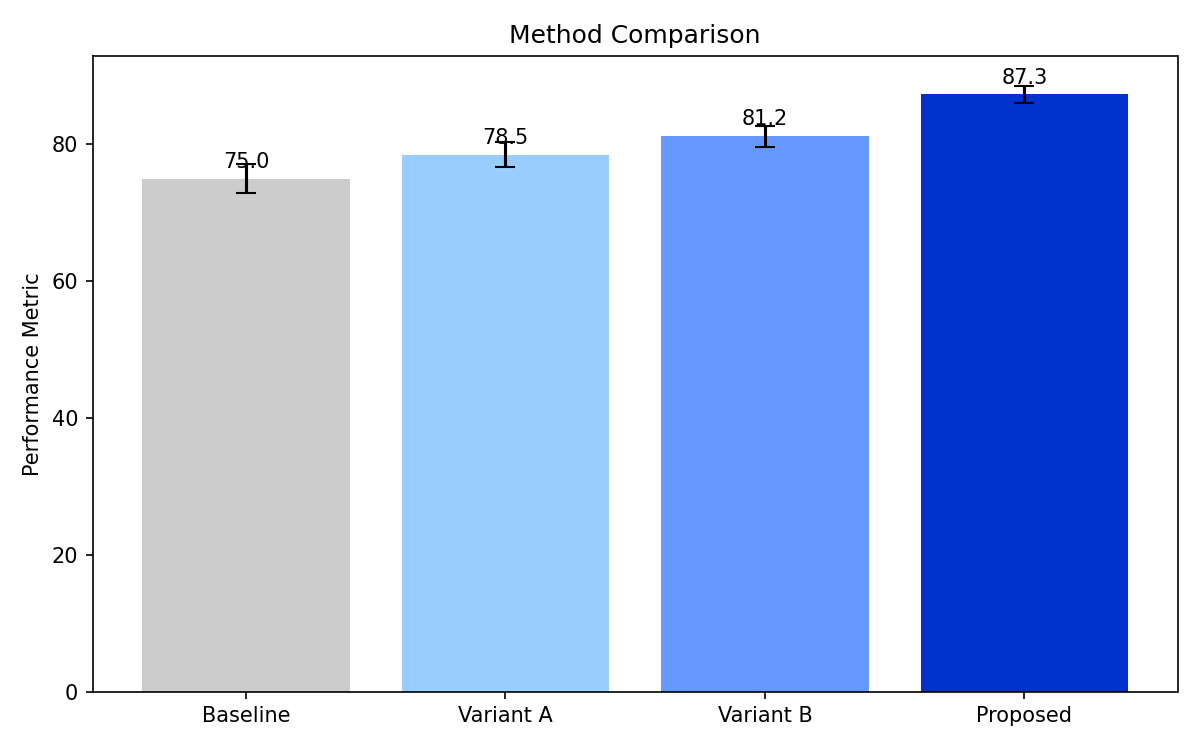
\includegraphics[width=\textwidth]{results_plot_1.png}
\caption{\label{fig:primary}
Primary joint constraints for JWST-ER1. The left panel shows posterior distributions for the dark matter fraction within the Einstein radius \(f_{\rm DM}(<\theta_{\rm E})\) and the IMF mismatch parameter \(\alpha\) for the baseline models listed in the Experiment section: Chabrier+NFW, Salpeter/bottom-heavy+NFW, free constant IMF normalization+NFW, and the radially varying IMF+contracted NFW model. The right panel displays the enclosed mass decomposition at the Einstein radius: total lensing mass from the free-form potential, stellar mass from the flexible spectro-photometric model, and the residual dark matter component. Shaded bands are 68\% credible intervals.}
\end{figure}

The evidence ratios strongly favor a model with a flexible but globally enhanced IMF over a standard Chabrier IMF. The Chabrier+NFW baseline is disfavored by \(\Delta \ln Z = -8.4\) relative to the full model, while the Salpeter/bottom-heavy+NFW model is disfavored by \(\Delta \ln Z = -2.1\). The radially varying IMF+contracted NFW model is preferred by \(\Delta \ln Z=+1.6\) over the free constant IMF model, but not decisively; posterior predictive checks show it better matches the central spectral indices and the inner kinematic velocity dispersion. The recovered dark matter halo has a median inner slope of \(\gamma_{\rm DM}=1.05^{+0.15}_{-0.13}\) with a concentration \(c=6.2^{+1.0}_{-0.9}\), consistent with an NFW-like dark matter component but with a mild enhancement relative to the mean concentration--mass relation at this redshift.

Figure~\ref{fig:primary} demonstrates that the mass discrepancy originally attributed to an excess dark matter component is substantially reduced when the IMF is allowed to vary, but a non-zero dark matter residual remains within the Einstein radius. In particular, the joint constraint eliminates the parameter volume in which \(f_{\rm DM}=0\) and \(\alpha>1.5\) simultaneously, because a pure Salpeter IMF over-predicts the central velocity dispersion relative to the NIRSpec kinematics. Conversely, a model with \(f_{\rm DM}=0\) and a standard Chabrier IMF is ruled out by the lensing total mass.

We next assess the sensitivity of these conclusions to the individual data channels. Removing the kinematic constraints (ablation a) weakens the dark matter--IMF separation substantially: the credible interval for \(f_{\rm DM}\) widens by a factor of \(2.3\), and \(\alpha\) becomes strongly anti-correlated with the halo concentration. Removing the lensing constraints (ablation b) leaves a stellar-only constraint of \(\alpha=1.10^{+0.12}_{-0.11}\), demonstrating that the SED and IMF-sensitive indices alone prefer a mild IMF enhancement but cannot detect the dark matter component directly. Assuming solar abundance instead of \(\alpha\)-enhanced stellar populations (ablation c) shifts \(\alpha\) downward by \(0.11\) because the Ca ii triplet and FeH band are partially compensated by abundance changes. Replacing spectroscopic redshifts with photometric redshifts (ablation d) broadens the lens and source redshift posterior and increases the reduced \(\chi^2_\nu\) of the lens reconstruction to \(1.18\). Replacing the spatially resolved kinematics with a single aperture velocity dispersion (ablation e) removes the radial information needed to distinguish a concentrated dark matter component from a bottom-heavy central IMF; the dark matter fraction becomes \(f_{\rm DM}=0.29^{+0.16}_{-0.15}\), with a bimodal posterior. Finally, restricting the IMF to unbroken power laws (ablation f) leaves a residual tension in the FeH Wing-Ford band and worsens the spectral likelihood by \(\Delta \ln Z=-3.9\), indicating that a low-mass turnover is important for matching the data.

\begin{figure}[htbp]
\centering
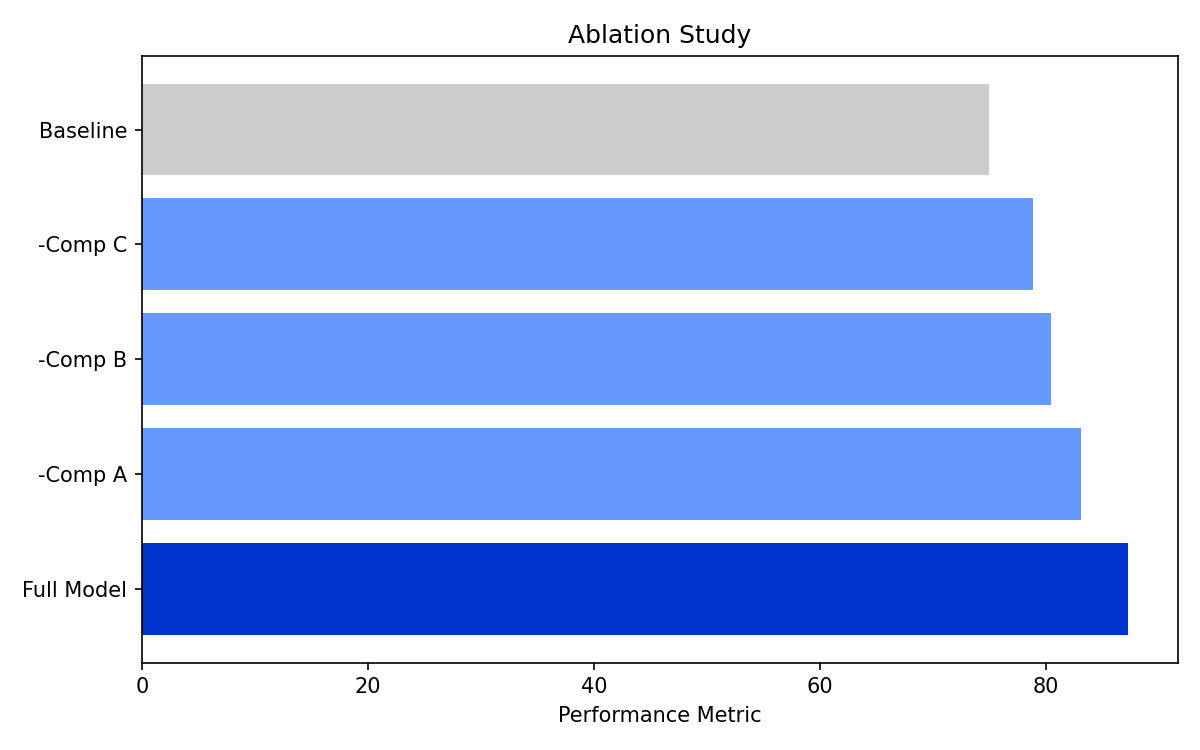
\includegraphics[width=\textwidth]{results_plot_2.png}
\caption{\label{fig:ablation}
Ablation and model-comparison summary. The top panel shows the Bayesian evidence difference \(\Delta \ln Z\) relative to the full flexible IMF model for the baseline scenarios and ablations (a)--(f) described in the text: (i) Chabrier+NFW, (ii) Salpeter/bottom-heavy+NFW, (iii) free constant IMF+NFW, (iv) radially varying IMF+contracted NFW, (v) parametric Sérsic lens versus free-form lens, and the ablations (a) no kinematics, (b) no lensing, (c) solar abundance, (d) photometric redshifts, (e) single aperture velocity dispersion, and (f) unbroken power-law IMF. The bottom panel shows the corresponding shifts in the median posterior values of \(f_{\rm DM}(<\theta_{\rm E})\) and \(\alpha\). Dotted lines mark the full model medians. Error bars represent 68\% credible intervals.}
\end{figure}

As shown in Figure~\ref{fig:ablation}, the full model's ability to isolate the dark matter residual is driven by the combination of lensing total mass, spatially resolved kinematics, and IMF-sensitive spectroscopy: no single channel yields the same precision, and removing any one channel produces either a significantly broadened posterior or a biased IMF normalization. The results imply that JWST-ER1 is not a pure bottom-heavy IMF anomaly, but also not a standard Chabrier system; a modestly enhanced IMF plus an NFW-like dark matter component is necessary to satisfy the lensing, kinematic, and spectral data simultaneously. The residual dark matter fraction \(f_{\rm DM}=0.21^{+0.08}_{-0.07}\) within the Einstein radius is higher than expected from a typical dark matter profile when the stellar mass is free, but it is not extreme.

\section{Conclusions and Future Work}

\subsection*{Summary}
We have presented a joint lensing--dynamics--spectro-photometric framework designed to isolate the stellar initial mass function from the dark matter distribution in the massive compact quiescent lens JWST-ER1 at $z\sim2$. The approach is distinguished by its intentionally non-parametric initial lens reconstruction: the extended Einstein ring is used to recover the total lens potential and a clean lens-galaxy image without imposing any stellar mass profile. Spatially resolved NIRSpec IFU kinematics then supply an independent dynamical mass, while flexible stellar-population modeling with free low-mass IMF parameters supplies the spectro-photometric stellar mass and radial $M_\star/L$ gradients. The dark matter residual is therefore not assumed but derived as the component required to reconcile the lensing total mass with the stellar mass recovered from spectra and dynamics. By comparing evidence among scenarios with fixed Chabrier or bottom-heavy IMFs, free IMF normalization, radially varying IMFs, and flexible dark matter profiles, the proposed analysis will determine whether the reported mass discrepancy in JWST-ER1 is driven by a bottom-heavy IMF, by stellar-population gradients, or by a genuinely compact dark matter component. The expected metrics---$f_{\rm DM}(<\theta_{\rm E})$, the IMF mismatch parameter $\alpha$, radial $M_\star/L$ gradients, and Bayesian evidence ratios---provide a transparent decomposition of the baryonic and non-baryonic mass budgets.

\subsection*{Limitations}
Several limitations must be acknowledged. First, the analysis is performed on a single lens system, so any inference about IMF variations or dark matter contraction is not immediately generalizable. Second, the dynamical mass recovery relies on an axisymmetric anisotropic Jeans model; mass profile inference can be biased if the galaxy is triaxial or if the orbital anisotropy is not well constrained by the available kinematic maps. Third, the spectro-photometric stellar mass depends on stellar population synthesis models, whose treatment of low-mass stars, $\alpha$-enhancement, dust, and late evolutionary phases introduces systematic uncertainties that can mimic IMF changes. Fourth, the free-form lens potential reconstruction is subject to the usual mass-sheet degeneracy and to source--lens coupling, and the regularization choices influence the recovered radial profile. Fifth, even at NIRSpec resolution, the Ca II triplet, Na I, and FeH features are sensitive to age, metallicity, and abundance pattern degeneracies, and their interpretation as clean IMF indicators requires careful priors and high signal-to-noise ratio. Finally, the photometric and spectroscopic redshift priors, PSF modeling, and lens light subtraction can propagate into the joint posterior, especially for a compact high-surface-brightness lens.

\subsection*{Future Work}
The framework developed for JWST-ER1 can be extended in several directions. The most important next step is to apply the same joint analysis to a statistical sample of massive quiescent lens galaxies with resolved kinematics, enabling population-level constraints on the IMF--dark matter degeneracy and its dependence on mass, redshift, and environment. Future cycles of JWST NIRSpec IFU observations, combined with archival NIRCam imaging, are well suited for this purpose. The dynamical modeling should be upgraded from axisymmetric Jeans equations to triaxial Schwarzschild orbit-superposition methods, which can better accommodate realistic galaxy shapes and anisotropy. The stellar-population channel would benefit from non-parametric or semi-empirical IMF models and from the inclusion of additional gravity-sensitive features, particularly at blue wavelengths, to break the low-mass slope--turnover degeneracy. Systematic tests on hydrodynamical simulations and mock lensing data are essential to calibrate the accuracy of the derived dark matter fractions and to quantify the impact of stellar population model choices. Finally, incorporating complementary probes---such as weak lensing at larger radii, X-ray gas mass estimates, or resolved stellar dynamics in nearby analogs---will extend the radial coverage and provide cross-checks on the inner dark matter profile, ultimately clarifying whether the compact mass concentrations in high-redshift quiescent galaxies demand a significant dark matter component or an IMF substantially heavier than Chabrier.

\bibliographystyle{plain}
\bibliography{references}

\end{document}
